\section{Detector and Shield Design}
\label{secDetectorDesign}

A total amount of 161~kg of LXe is enclosed in the vacuum insulated cryostat, made from the low activity stainless steel of type 1.4571/316Ti (316Ti SS). The target consists of 62~kg of LXe, defined by a structure made from polytetrafluoroethylene (PTFE, {\it Teflon}) and copper.
The target volume is viewed by two arrays of photomultiplier tubes (PMT), one on the bottom immersed in LXe, and one in the gas phase above the target volume.
The electric fields of the TPC are generated by applying potential differences across the electrodes, which are made of stainless steel meshes welded onto 316Ti SS rings. They include two electrodes on the bottom of the TPC above the bottom PMT array, and a stack of three electrodes around the liquid-gas interface.

The passive shield is shown in Fig.~\ref{figXe100shield_1}. It encloses the detector in 4$\pi$, and is installed on a 25~cm slab of polyethylene. From outside to inside, it consists of tanks filled with water (thickness 20~cm, Fig.~\ref{figXe100shield_2}) to shield against ambient neutrons, placed on three sides and on top of the shield. After the water shield, there are two layers of lead: a 15~cm outer layer and a 5~cm inner layer, which has a low contamination of the radioactive isotope ${^{210}}$Pb (Section~\ref{secDetectorMaterials}). Inside the lead, there are 20~cm of polyethylene to shield against further neutron backgrounds. The innermost shield layer consists of 5~cm thick (0.5~cm on the bottom) copper plates. It reduces the gamma background from the outer shield layers. The inner shield cavity is constantly purged with high purity boil-off nitrogen at a rate of $\sim$17~standard liters per minute (slpm) in order to avoid penetration of radon. Detector components with relatively high radioactive contamination are mounted outside of the shield, for example signal and high voltage feedthroughs, vacuum pumps, pressure sensors and associated electronics. An important detector design feature, which has contributed to the low background rate of XENON100, is `remote cooling' - the installation of the cryogenics system, based on a pulse tube refrigerator (PTR)~\cite{PTR}, outside the passive shield, far away from the xenon target.

\begin{figure}[!h]
\centering
\subfigure[]{
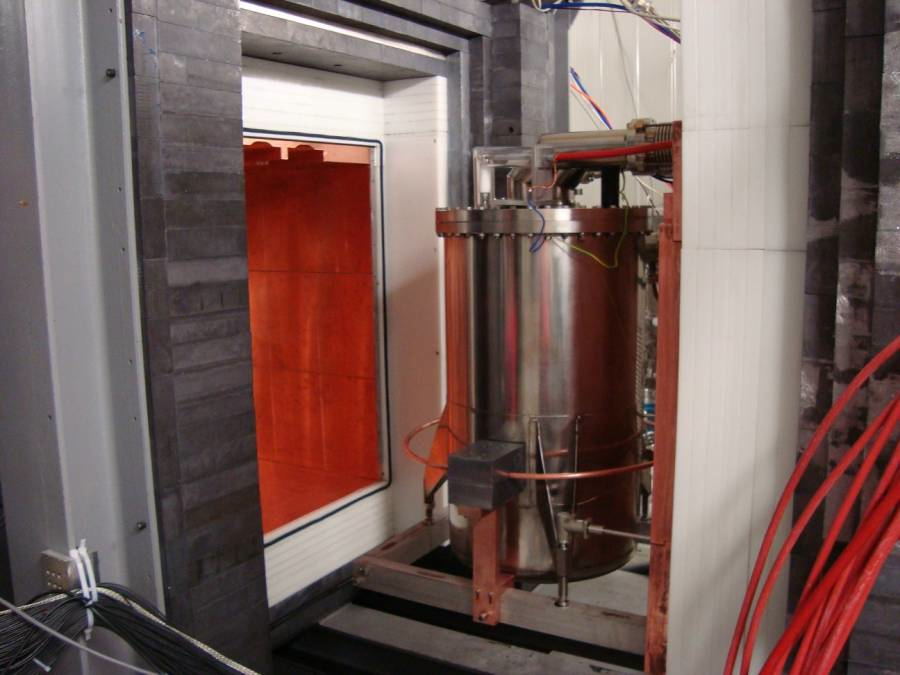
\includegraphics[height=0.45\linewidth]{plots/Detector/Xe100shield.png}
\label{figXe100shield_1}}
\subfigure[]{
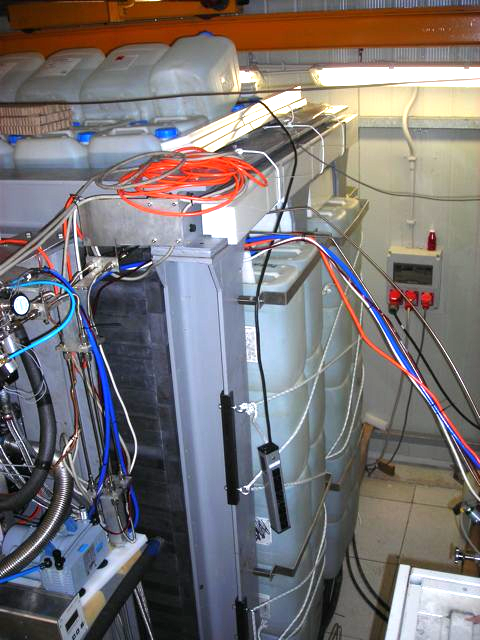
\includegraphics[height=0.45\linewidth]{plots/Detector/WaterShield.png}
\label{figXe100shield_2}}
\caption[The XENON100 detector with the open shield door, and the water shield]{The XENON100 detector with the open shield door (a), and the water shield (b).}
\label{figXe100shield}
\end{figure}

The schematic drawing of the XENON100 detector is shown in Fig.~\ref{figXe100CAD}.
The quasi-cylindrical TPC is formed by 24 interlocking PTFE panels with a thickness of 6.35~mm, see also Fig.~\ref{figTPC}. PTFE reflects scintillation light with high efficiency~\cite{yamashita}, and optically separates the 62~kg target volume from the surrounding liquid xenon, which is in average 4~cm thick and has a total mass of 99~kg. This allows exploitation of the self-shielding capability of liquid xenon due to its high density (2.83~g/cm$^{3}$ at T = 182~K, P = 2.3~atm) and high atomic number ($Z$ = 54). In addition, this volume around the target is instrumented with PMTs, becoming an active veto for background reduction by rejecting events in which a particle deposits part of its energy in the veto volume. 

\begin{figure}[!t]
\centering
%\includegraphics[width=1.0\linewidth]{plots/Detector/Xe100_CAD_withLabels2.png}
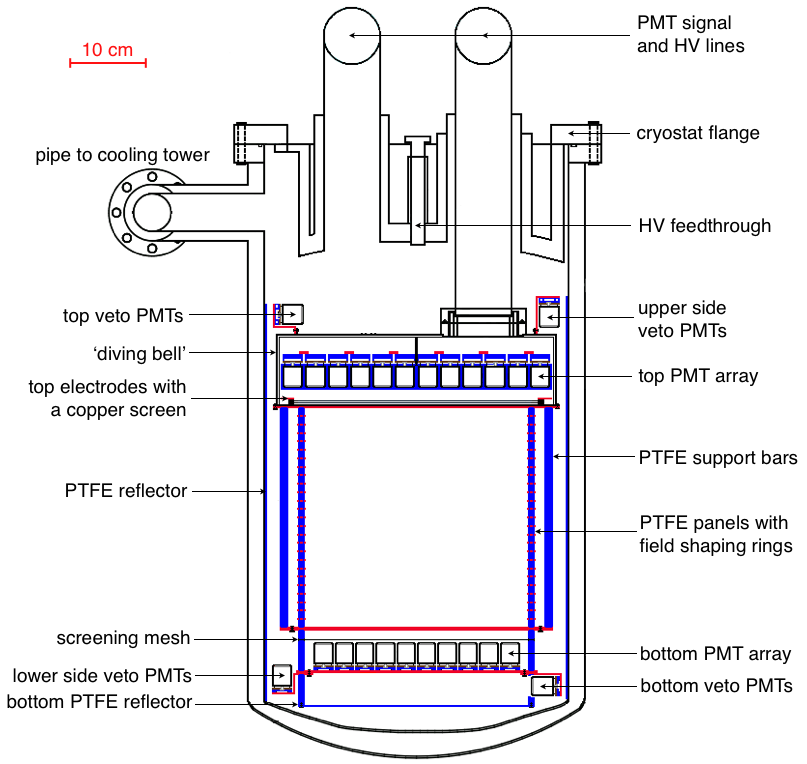
\includegraphics[width=1.0\linewidth]{plots/Detector/Xe100_CAD_withLabelsAndScale.png}
\caption[Schematic view of the XENON100 detector]{Schematic view of the XENON100 detector. The colors show: black - stainless steel, red - copper, blue - PTFE. Figure published in Ref.~\cite{xe100-instrument}.}
\label{figXe100CAD}
\end{figure}

\begin{table}[!t]
\centering
\caption[Thickness of the 316Ti stainless steel used for different detector components, and their weight]{Thickness of the 316Ti stainless steel used for different detector components, and their weight. The support rings for the top electrodes are milled down to 2.5~mm from 3.0~mm plates.}
\label{tabStainlessSteel}
\vspace{0.2cm}
\begin{tabular}{>{\footnotesize}l|>{\footnotesize}l|>{\footnotesize}c}
%\begin{tabular}{l|l|c}
\hline
Detector component 					& Steel thickness [mm]		& Weight [kg] \\
\hline
Inner cryostat vessel						& 1.5 					& 12.2 \\
Outer detector vessel					& 1.5						& 14.1 \\
Cryostat lid with the top pipes				& 1.5						& 30.8 \\	
Flange								& 25.0					& 12.8 \\
Diving bell							& 2.5						& 3.6 \\
Support ring for the cathode 				& 1.5						& 0.074 \\
Support ring for the screening mesh			& 3.0						& 0.156 \\
Three support rings for the top electrodes 	& 3.0 					& 0.24 \\
Cryostat support bars					& 25.0					& 49.68 \\
\hline
\end{tabular}
\end{table}

%The cryostat and some other parts of the detector are made from austenitic stainless steel of type 316Ti in AISI standard~\cite{316Ti}.
Steel plates of various thickness have been used for different detector components, with different radioactive contaminations (details in Section~\ref{secScreening}). The thickness of the 316Ti stainless steel and the corresponding weight of the detector components are shown in Table~\ref{tabStainlessSteel}. The total weight of the cryostat vessel is 70.0~kg, which is only 30\% of that of the XENON10 detector's cryostat~\cite{xe10-instrument}. 
The cryostat is supported inside the shield by 316Ti SS bars, which are mounted onto the movable shield door (Fig.~\ref{figXe100shield_1}). 

The inner vessel containing the LXe is lined on the walls and the bottom with a 1.5~mm thick PTFE layer  in order to increase the light collection efficiency in the active veto volume. The pipes guiding PMT signal and high voltage cables have been designed to be single wall to reduce the amount of radioactive material close to the detector.

Electrons created by ionization in the LXe target are drifted upwards by an electric field created by applying voltage on the cathode, a 75~$\mu$m thick stainless steel mesh with hexagonal structure with a 5~mm pitch, installed on the bottom of the TPC. The initial design has foreseen to use a high voltage of $-$30~kV to generate a drift field of 1~kV/cm. Electron field emission and subsequent scintillation in the strong electric field around the cathode wires resulted in induced single photoelectron-like events in the waveforms. As a result, the operation voltage has been lowered to $-$16~kV for stable operation, which corresponds to a drift field across the TPC of 0.53~kV/cm. In order to shield the bottom PMTs from this electric field, an additional grounded electrode (50~$\mu$m mesh) is installed below the cathode.

\begin{floatingfigure}[l]{0.45\textwidth}
%\begin{figure}[!h]
\centering
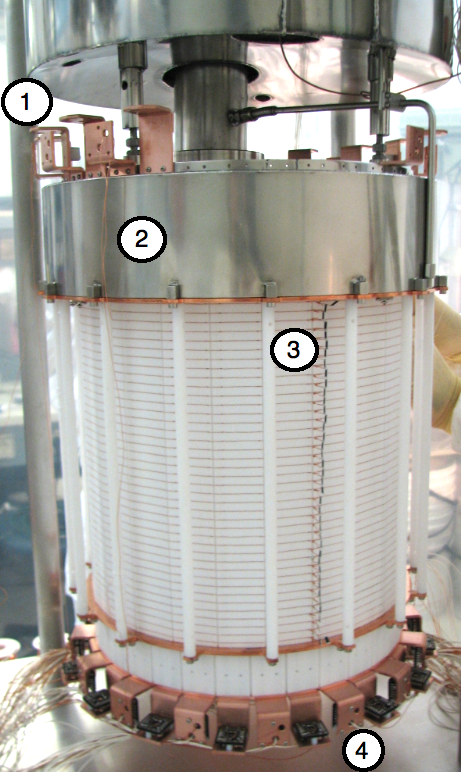
\includegraphics[height=0.65\linewidth]{plots/Detector/TPC_withLabels.png}
%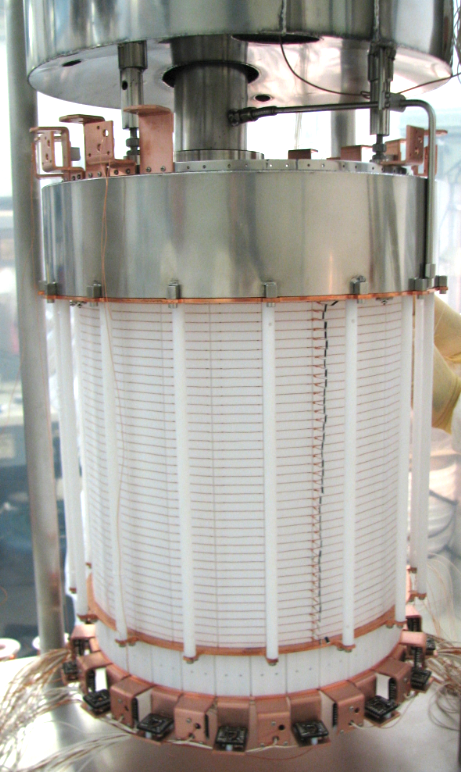
\includegraphics{plots/Detector/TPC.png}
\caption[The XENON100 time-projection chamber]{The XENON100 TPC during detector assembly in the clean room: 1- copper angles for the top and upper side veto PMTs, 2 - `diving bell', 3 - resistor chain connecting the field shaping rings, 4 - copper angles for the bottom and lower side veto PMTs.}
\label{figTPC}
%\end{figure}
\end{floatingfigure}

The gas phase for charge amplification via proportional scintillation is maintained using a `diving bell' system, made from 316Ti SS with a total weight 3.6~kg. It allows the liquid level to be kept constant at a precise height while having an additional layer of LXe above the TPC. A slight overpressure in the bell is provided by the gas returning from the continuous recirculation system.
The liquid level is adjusted by changing the recirculation rate, and by adjusting the height of the gas outlet from the bell by a motion feedthrough.

An extraction field is created across the liquid-gas interface by applying high voltage on the anode, 125~$\mu$m mesh with 2.5~mm pitch, which is placed inside the diving bell. The value of the extraction field depends on the position of the liquid-gas interface, which is adjusted to give $\sim$12~kV/cm in the gas phase at +4.5~kV applied to the anode. This field is high enough to obtain an extraction efficiency close to 100~\%~\cite{ExtractionField}. 
Two additional electrodes are installed below and above the anode and are kept at ground potential in order to close the field cage and shield the top PMT array from the high electric field.  The gaps between the top electrodes are 5~mm, and the liquid level is adjusted between the lower two of them. The entire stack of the top electrodes is optimized for optical transparency and minimal impact on the S2 resolution.

The scintillation light is detected by 242 one square inch R8520-06-AL Hamamatsu PMTs. They are among the PMTs with the lowest measured radioactivity (see Section~\ref{secScreening}), and are optimized for operation in LXe (at T = 182~K, P = 2.3~atm). 
The top PMT array consists of 98 PMTs in a PTFE support structure inside the diving bell, and 80 PMTs are installed below the cathode in the LXe. Additionally, 64 PMTs are mounted on copper angles and view liquid xenon of the veto volume.

%(milled from 3.0 SS plates)
%`
